\section{Ajout de fonctionnalités}

\subsection{L'implémentation du retour sonore}
\paragraph{}
Dans le programme de Jérémy Lixandre, la classe \verb!Parser! a pour
utilité de récupérer les informations du fichier de configuration
\verb!config.cfg!, notamment toutes les fonctions de
\textit{processing}. Ce fichier a donc été modifié afin de prendre en
compte notre nouvelle fonction de \textit{processing}, la fonction de
mixage, qui vient s'ajouter aux trois existantes. Tout comme ces
fonctions, elle est générique et doit pouvoir être sélectionnée par
l'utilisateur depuis un menu de configuration.

\paragraph{}
Un fichier dédié à la fonction de mixage a un nom commençant par
\verb!Mix!. Il est répertorié dans le dossier \verb!Mix! du dossier
\verb!Process!. La fonction de mixage doit prendre une matrice en
paramètre ; il s'agit de la matrice retournée par la fonction de
calcul du coefficient de corrélation. Elle retourne un vecteur de
coefficients : à un instant donné, chaque piste dispose désormais d'un
seul coefficient qui doit déterminer la façon dont elle va être
diminuée en volume sonore dans le retour audio.

\paragraph{}
Nous avons implémenté plusieurs fonctions de mixage. La fonction
\verb!vector<float>!
\\ \verb!MixMaxCorrelated!, par
exemple, renvoie un coefficient égal à la moyenne des coefficients de
corrélation de la piste avec toutes les autres pistes. Les instruments
les moins corrélés recevront ici un malus sur l'amplitude de leur signal.
Tandis que la fonction de traduction du coefficient de corrélation en
triplet RGB est dédiée uniquement au retour visuel, celle de mixage est
dédiée uniquement au retour sonore.

\begin{lstlisting}[language=C, frame=single, breaklines=true]
vector<float> MixMaxCorrelated(const Matrix<float>& correlMatrix){

  int row = correlMatrix.getSize();
  int col = correlMatrix.getRow(0).size();

  // initialize the result vector with zeros
  vector<float> meanCorrelations(row, 0.0f);

  // fill the vector with the mean correlation of
  // each instrument with others
  for (int i = 0; i < row; i++) {
    for (int j = 0; j < col; j++) {
      if (i != j)
        meanCorrelations[i] += correlMatrix.getCase(i, j);
    }
    meanCorrelations[i] /= (float)row-1;
  }
  return meanCorrelations;
}
\end{lstlisting}

\begin{center}
 \textit{Ci-dessus, l'exemple de la fonction de mixage précédemment cité}
\end{center}

\paragraph{}
Dans la fonction \verb!void parseProcessFunc!  appelée dans le fichier
\verb!main.cpp!, nous avons dû ajouter l'analyse de la fonction de
mixage sur le modèle des analyses des trois autres fonctions de
\textit{processing}.

\paragraph{}
L'architecture de Bela a été conçue pour permettre la synthèse d'un
retour sonore dans le corps de la fonction \verb!void render! du
fichier éponyme. Grâce au code implémenté par notre prédécesseur au
sein de cette fonction, Bela peut synthétiser un retour sonore modifié
par notre fonction de mixage.

\begin{lstlisting}[language=C, frame=single, breaklines=true]
for(unsigned int i=0; i<context->audioOutChannels; i++){
   if(gSampleFactor == STANDARD_SAMPLE_RATE){
      audioWrite(context, 2 * n, i, out);
      audioWrite(context, 2 * n + 1, i, out);
   } else {
      audioWrite(context, n, i, out);
   }
}
\end{lstlisting}

\begin{center} \textit{Ci-dessus, l'implémentation du retour sonore
  dans le corps de la fonction principale de \verb!render.cpp!. Via la
  fonction \verb!audioWrite!, la variable \verb!out! récupère un à un
  les signaux de chaque type de piste sonore
  (audio/analogique/digitale) multipliés par la moyenne de leurs
  coefficients de corrélation par rapport aux autres
  signaux.} \end{center}

 \paragraph{}
 Dans le fichier \verb!render.cpp!, la fonction
 \verb!void processBuffer()! est utilisée comme tâche auxiliaire de la
 boucle de traitement principale. Nous avons déclaré un vecteur
 \verb!gMeanCorrel! dans \verb!render.cpp! ; initialisé avec une valeur
 de 1 pour tous les indices, il prend la valeur que retourne la
 fonction de mixage à l'intérieur du code de la fonction
 \verb!void ProcessMultiCorrel::process!
 que nous avons modifiée et qui est appelée dans \verb!processBuffer!
 de \verb!render.cpp!.
 \paragraph{}
 Dans l'implémentation de Jérémy Lixandre, le traitement des tâches
 auxiliaires dans \verb!render.cpp! se faisait à sens unique
 (exécution de tâches auxiliaires sans retour de valeur dans la boucle
 de traitement principale). Afin de récupérer le résultat du
 traitement de la fonction de mixage, nous avons passé la référence du
 vecteur contenant les moyennes de coefficients de corrélation,
 \verb!gMeanCorrel!, en paramètre de la fonction
 \verb!ProcessMultiCorrel::process! lors de son appel dans la fonction
 principale de \verb!render.cpp!. On accède ainsi à la case mémoire de
 la variable pour permettre à la fonction de modifier son contenu et
 ainsi d'affecter les valeurs de retour de la fonction de mixage au
 vecteur ; c'est ainsi que la modification des volumes devient
 possible.

 \begin{lstlisting}[language=C, frame=single, breaklines=true]
void ProcessMultiCorrel::process(const Matrix<float>& buffer,
                                 vector<float>& meanCorrelations,
                                 Connection conn){
  Matrix<float> copy = buffer;

  // Processing functions
  copy = _preprocess(buffer);
  Matrix<float> correlMatrix = calcul_correl(copy);
  process_volume(correlMatrix, meanCorrelations);
  Matrix<RGB> mat = color_matrix(correlMatrix);

  // Send data
  string str = mat.toString();
  conn.send(str);
}
 \end{lstlisting}
 \begin{center}
  \textit{L'appel de la fonction \verb!process! ci-dessus exécute une série de fonctions de traitement de manière séquentielle.}
 \end{center}

 \begin{lstlisting}[language=C, frame=single, breaklines=true]
  void ProcessMultiCorrel::process_volume(const Matrix<float>&
                                            correlMatrix,
                                            vector<float>&
                                            meanCorrelations){
    meanCorrelations = this->_mixLevel(correlMatrix);
  }
 \end{lstlisting}
 \begin{center}
  \textit{Ci-dessus, la fonction appelée dans le corps de la fonction \verb!process!. Nous l'avons implémentée de sorte à altérer en son sein la valeur du vecteur des moyennes de corrélation passé par référence en paramètre.}
 \end{center}

 \subsection{L'interface de configuration utilisateur}
 \paragraph{}

 \subsubsection{Présentation de l'architecture}
 Afin d'implémenter l'interface de configuration utilisateur
 précédemment abordée nous avons ajouté à l'architecture du programme
 un dossier \verb!GUI! (\textit{Graphic User Interface}) à la racine
 du programme.  Le sous-répertoire contenant les fichiers relatifs à
 l'implémentation de l'interface de configuration se nomme
 \verb!settingWindow!.

 \begin{figure}[h]
  \centering
  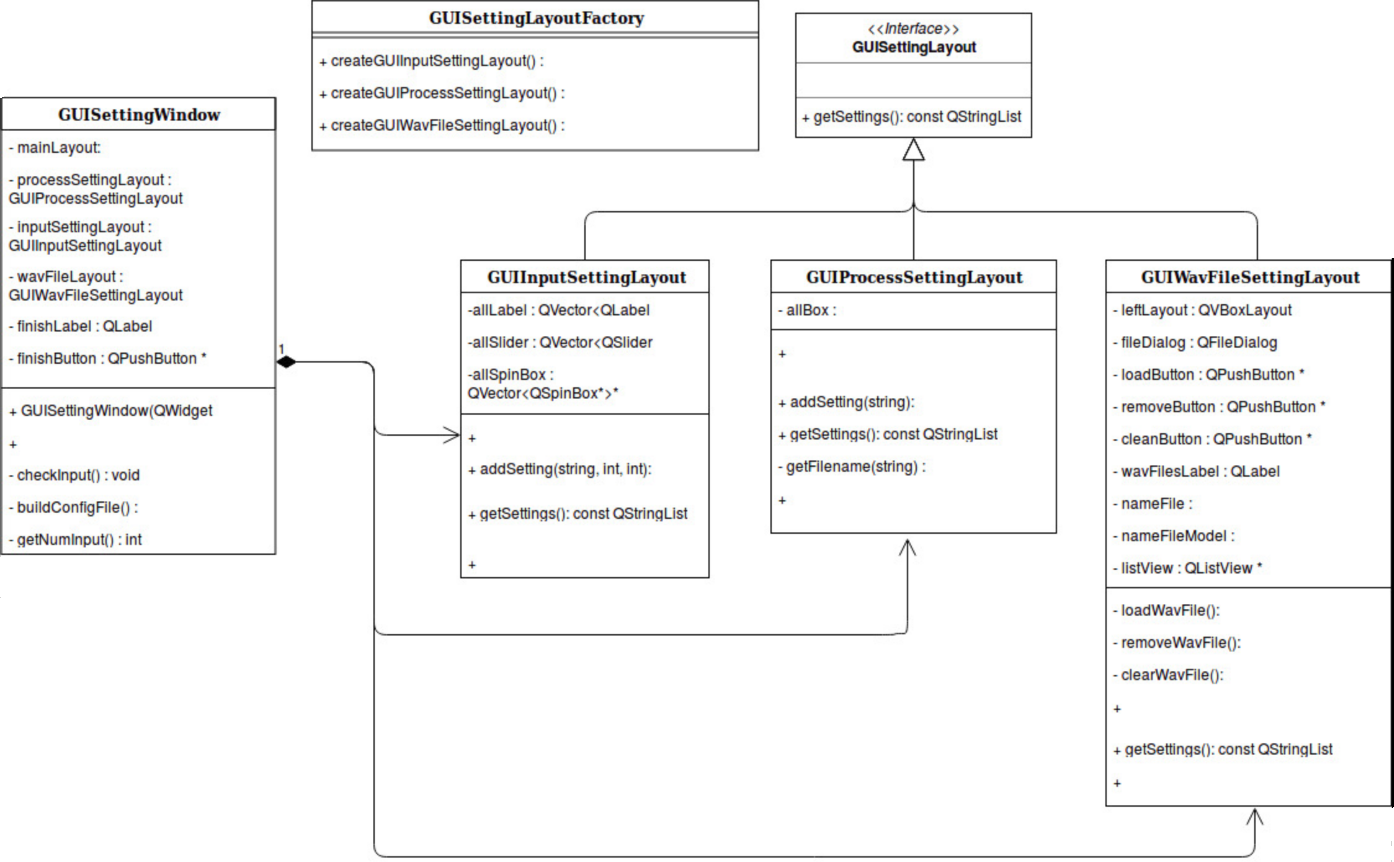
\includegraphics[scale=0.3]{assets/umlSettingWindow.png}
  \caption{Schéma global du dispositif de VisualImpro}
  \label{schéma global}
 \end{figure}


 \paragraph{}
 La classe principale de cette interface de configuration est la
 classe \verb!settingWindow!. Elle constitue une fenêtre vide
 destinée à afficher les données suivantes via un layout principale :
 \begin{itemize}
  \item Paramètres de fonction de traitement.
  \item Paramètres du nombre d'entrées audio et analog.
  \item Choix des fichiers audio \textit{.wav}.
 \end{itemize}
 Afin de créer de pouvoir créer ces parties, la fenêtre se sert d'une factory,
 % a AJOUTER
 - la factory permet de créer toutes les parties.
 -dans chaqu'un des layout la fenetre principale peut ajouter un paramètre a chaque
 partie.
 -chaqu'une des parties permet d'extraire un resultat precis : input pour recuperer un nombre
 process pour nom de fonction,wav pour fichier wav.
 -une fois que tout les paramètres , la fenetre va les recuperer et creer un
 fichier de sortie a laide d'un builder.
 -le builder sert a crée un fichier de sortie suivant un certains format. Dans le
 futur on pourra s'en servir pour creer un nouveaux format de retour pour pouvoir
 se passe du fichier config.
 -dans notre cas le type de fichier est un fichier cfg qui sera envoyer a bela.

 \subsubsection{Fonctionnement de chaque classe}
 \paragraph{}
 -classe setting window contient tout les layouts et un bouton fin quand tout les
 parametre sont mis. le nombre d'input doit etre superieur ou egal a 2 car sinon pas de
 correlation.
 - toute les classes layout herite de GUISettingLayout qui possede la fonction
 abstract getSettings qui permet de retourner tout les parametre selectionné dans le layout.
 -inputSettinLayout contient pour chacune de ses sous parties un slider et une box
 pour pouvoir selectionné un nombre. Le nombre selectionné est compris entre un
 minimum et un maximum initialisé a la creation de la partie.
 -wavfilesetting permet de chercher des fichiers wav et de stocker leurs chemin
 absolut
 -processSetting va chercher, dans un dossier portant un nom egale au nom données
 en paramètre, les fichiers portant le nom de ce dossier, ou il y a une fonction
 et permettra de choisir la fonction que l'utilisateur voudra.



 \begin{figure}[h]
  \centering
  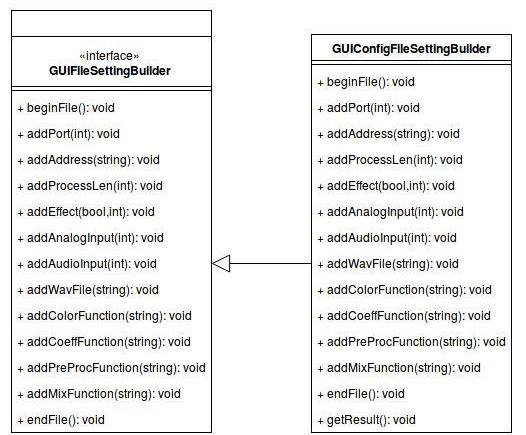
\includegraphics[scale=0.5]{assets/umlBuilder.png}
  \caption{Schéma global du dispositif de VisualImpro}
  \label{schéma global}
 \end{figure}

 \paragraph{}
 La fenêtre de configuration%AJOUTER

 \subsection{Autres ajouts mineurs sur le programme}
 \paragraph{}
 Nous avons implémenté une nouvelle fonction de corrélation dédiée aux
 tests : appelée \verb!CoeffRandom!, elle établit un coefficient de
 corrélation de manière aléatoire. La généricité de l'implémentation
 existante a rendu la tâche triviale, il nous a suffi d'écrire un
 fichier d'en-tête \verb!CoeffRandom.hpp! et un fichier source
 \verb!CoeffRandom.cpp! dans le dossier \verb!Coeff! contenant les
 fonctions de calcul du coefficient de corrélation (dossier
 \verb!process!). Cette fonction renvoie un flottant compris entre 0 et
 1, comme les autres fonctions de corrélation. L'accomplissement de
 cette tâche et la trivialité qu'il représente témoigne de la
 généricité des fonctions de corrélation, et des fonctions de
 traitement en général, qui possèdent désormais toutes plusieurs
 versions alternatives.
